\section{Implementation}

Although the paper gives a continuous formulation of the problem, in practice we must discretize the representation of the shape. We use a 2D triangular mesh that encompasses the used image. The image is then used as a texture for the mesh. 

In order to provide the so-called "keyframes," which are essentially complex transformations of the vertices in the original mesh to a new set of vertices comprising the new mesh, we use the method by [Chen \& Weber 2015]. We call these "keyframes" deformations of the original mesh. 

\subsection{Creating Deformations}

This method by Chen \& Weber is used to generate deformations of the input mesh so that the resulting mappings are of bounded distortion and harmonic. It is particularly important that these deformations be harmonic (or approximately harmonic, since we are discretizing the mapping). The intuition behind this is that harmonic mappings have low Dirichlet energy, which is a metric for how variable / distorted a function is. % why is harmonicity good? Recall that harmonic mappings have low Dirichlet energy (distortion)

These deformations are, as mentioned before, harmonic complex transformations $f$ of the mesh. So to find the resulting vertices, we simply take $f(v)$ for every complex coordinate vertex $v$ in the mesh. It will however, be convenient to represent this harmonic function $f$ as the sum of a holomorphic and anti-holomorphic function $\phi + \overline{\psi}$ as given in Equation \ref{eq:decomposition}. In turn, it is convenient to represent the holomorphic functions $\phi, \psi$ as Cauchy complex barycentric coordinates. These are, in short, the Cauchy coordinates.


\subsubsection{Cauchy Coordinates}

When speaking about a mesh, we can decompose holomorphic functions into the sum of Cauchy coordinates, or functions related to the vertices in the cage of the mesh.

\begin{figure}[h]
	\centering
	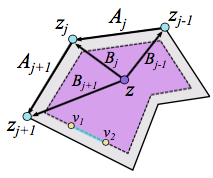
\includegraphics[width=0.25\textwidth]{Images/Cauchy-Cage.png}
	\caption{Cauchy Cage [Chen \& Weber 2015]}
	\label{fig:Cauchy-Cage}
\end{figure}

In this way, any holomorphic function $\Phi(z)$ can be written as:

$$\Phi(z) = \sum_{j=1}^n C_j(z) \phi_j$$

where $\phi_j$ is a complex constant.

\subsection{Creating Deformations (Continued)}

We assume the domain's boundary is a simply connected polygon $P$. We can offset the boundary in the outward normal direction to form the cage $\hat{P} = \{z_1, z_2, \ldots, z_n\}, z_i \in \mathbb{C}$. 

$\ldots$

Then after minimizing the ARAP energy in a series of loops, we obtain functions $\Phi, \Psi$ which comprise our mapping $f$. Recall that these functions are written as:

\begin{align*}
\Phi(z) &= \sum_{j=1}^n C_j(z) \phi_j \\
\Psi(z) &= \sum_{j=1}^n C_j(z) \psi_j
\end{align*}

where we know the complex numbers $\{\phi_1, \phi_2, \ldots, \phi_n\}, \{\psi_1, \psi_2, \ldots, \psi_n\}$ as well as the closed form representation of TO BE CONTINUED.


 
